\chapter{面向线性恢复的DSC辅助编码计算结果下行传输方法} \label{chapter-cooperative-transmission}

\section{引言}
在分布式机器学习场景中，大规模梯度计算往往会被划分为多个数据集分发给多个工作节点上执行。然而，由于一些工作节点可能成为迟滞节点，影响整体系统的收敛速度。为了缓解迟滞效应，梯度编码被提出作为应对迟滞效应的方法。一些工作主要研究了如何设计编码计算的方案，忽略了无线通信过程可能由于信道衰落造成的通信延迟。此外，同时考虑了计算和通信延迟的一些工作中，工作节点采用独立传输计算结果的方式，没有充分利用节点任务间由于任务编码引入的相关性。为了进一步提升梯度编码的传输效率，本章考虑引入DSC方案，对计算节点的计算任务进行压缩后传输，并达到负载重分配的效果。与上一章所述内容的区别在于，由于梯度编码场景中，移动设备只需要恢复工作节点的梯度和，不需要独立恢复所有工作节点的局部梯度值。如果继续采用经典SW定理进行压缩，移动设备需要独立恢复每个节点传输回来的计算结果再进行梯度求和，可能会造成信息冗余。
为了进一步传输效率，本章提出一种面向线性恢复的DSC辅助编码计算结果下行传输机制。具体来说，该机制采用基于嵌套线性码的信源编码方案，实现了比SW区域更大的压缩区域，使得梯度编码场景下可能会得到更好的传输效率。基于此，本章对所提出的下行传输机制建模了最小化传输时延优化问题，针对优化复杂度过高，后续将优化问题拆分成通用的优化子问题，并基于凹凸过程对优化问题进行求解，设计了相应的优化算法。

本章后续内容的安排如下：第\ref{4.2}节介绍了面向线性恢复的梯度编码计算下行传输模型；第\ref{4.3}节详细阐述了所提的面向线性恢复的DSC辅助编码计算下行传输机制；第\ref{4.4}节针对所提机制下的最小化传输时延问题进行求解，设计相应的优化算法；第\ref{4.5}节通过数值仿真实验结果对所提机制的效果进行验证；第\ref{chapter-sum}节对本章内容进行了总结。本章重要符号参见表\ref{<chapter-four-table-symbols>}。
\begin{table}
	%\small
	\centering
	\caption{本章常用符号}
	\begin{tabular}{c p{28em}}
		\toprule
		符号 & 含义 \\
		\midrule
	$k$ & 边缘节点数目 \\
	$r$ & 划分的子任务数目 \\
	$\mathcal{J}$&参与下行传输的边缘节点集合\\
	$X_i$ & 未编码子任务$i$的计算结果 \\
	$Y_i$ & 编码子任务$i$的计算结果 \\
	$S_{Y_i}$& 编码子任务$i$的计算结果对应生成的伴随式\\
	$S_{X_i}$& 未编码子任务$i$的计算结果对应生成的伴随式\\
	$\tilde{\eta}$ & 直接信源编码的压缩率 \\
	$\bar{\eta}$ & 理想信源编码的压缩率\\
	$\eta$ & 基于伴随式穿刺的实际信源编码的压缩率\\
	$s$ & 每个节点需要传输的符号数 \\
	$T_d$ & 下行传输所需时延 \\
	$P_{\text{max}}$ & 边缘节点的最大传输功率 \\
	$\symbfit{g}_i$ & 移动设备与边缘节点$i$间的信道增益 \\
	$B$ & 下行信道带宽 \\
	$n_0$ & 信道噪声功率谱密度 \\      
		\bottomrule
	\end{tabular}
	\label{<chapter-four-table-symbols>}
\end{table}

\section{系统模型与问题建模}\label{4.2}

考虑如图\ref{gradient coding_chapter}所示的梯度编码计算场景，包含一个移动设备和$N$个边缘节点$[N]={1,2,\cdots,N}$。移动设备将大规模模型训练任务$f(\mathcal{D})$卸载至这$N$个边缘节点上执行并行计算，其中，$\mathcal{D}$为训练数据集，假设训练数据集包含$v$个样本$\mathcal{D}={(x_1,y_1),\cdots,(x_v,y_v)}$，$f(\cdot)$表示梯度计算函数。考虑计算函数为通过最小化损失函数求解最优模型参数$w^*$，即$w^*=\arg \min_{w} \sum_{i=1}^v l(w;x_i,y_i)$，其中，$l(\cdot)$为样本损失函数。采用梯度下降算法时，在第$t$次迭代，系统需要计算全梯度$\mathbf{g}^{(t)}=\sum_{i=1}^v \nabla l(w^{(t)};x_i,y_i)$以更新模型。
为缓解分布式同步训练中由随机迟滞节点引发的迟滞效应，采用梯度编码技术\upcite{9755943}。梯度编码过程包含冗余数据分发与局部梯度计算两个阶段，由预先设计的编码矩阵$\mathbf{B}=[b_{n,k}]_{n\in[N],k\in[K]}$确定，其中编码矩阵$\mathbf{B}$可通过循环重复编码方案得到\upcite{tandon2017gradient}。具体而言，为降低单个节点的计算负载，原始数据集$\mathcal{D}$被划分为$K$个互不重叠的数据分块$\{\mathcal{D}_k\}_{k=1}^K$，分块后数据集的计算子任务可以表示为$\mathbf{g}_k=f(\mathcal{D}_k),k\in[K]$。以采用循环编码方案为例，编码矩阵$\mathbf{B}$的非零元素决定了分块数据集的分配，记为$\mathcal{I}_n=\{k\in[K]|B_{n,k}\neq0\}$，根据梯度编码理论，为容忍任意$S$个迟滞节点，每个数据分块必须被至少$S+1$个边缘节点持有，即编码矩阵$\mathbf{B}$的每一列至少包含$S+1$个非零元素，分后的计算子任务通过循环重复方案分发给$N$个边缘节点进行计算，每个边缘节点至少分配$S+1$个计算子任务。在每次迭代$t$中，边缘节点$n$首先计算本地持有数据分块的局部梯度$\left\{\mathbf{g}_i^{(t)}\right\}_{i\in \mathcal{I}_n}$，随后根据编码系数$b_{n,k},i\in[K]$计算局部梯度的线性组合，即
\begin{equation}
	\tilde{\mathbf{g}}_n^{(t)}=\sum_{k=1}^K b_{n,k}f(\mathcal{D}_k),
\end{equation}
其中，假设$\mathbf{g}_n^{(t)}$和$\tilde{\mathbf{g}}_n^{(t)}$中的元素定义在有限域$GF(q)$上，且为独立同分布的随机变量，$H(\tilde{\mathbf{g}}_n)$表示$\tilde{\mathbf{g}}_n^{(t)}$的信息熵。

\begin{figure}[htbp]
	\centering
	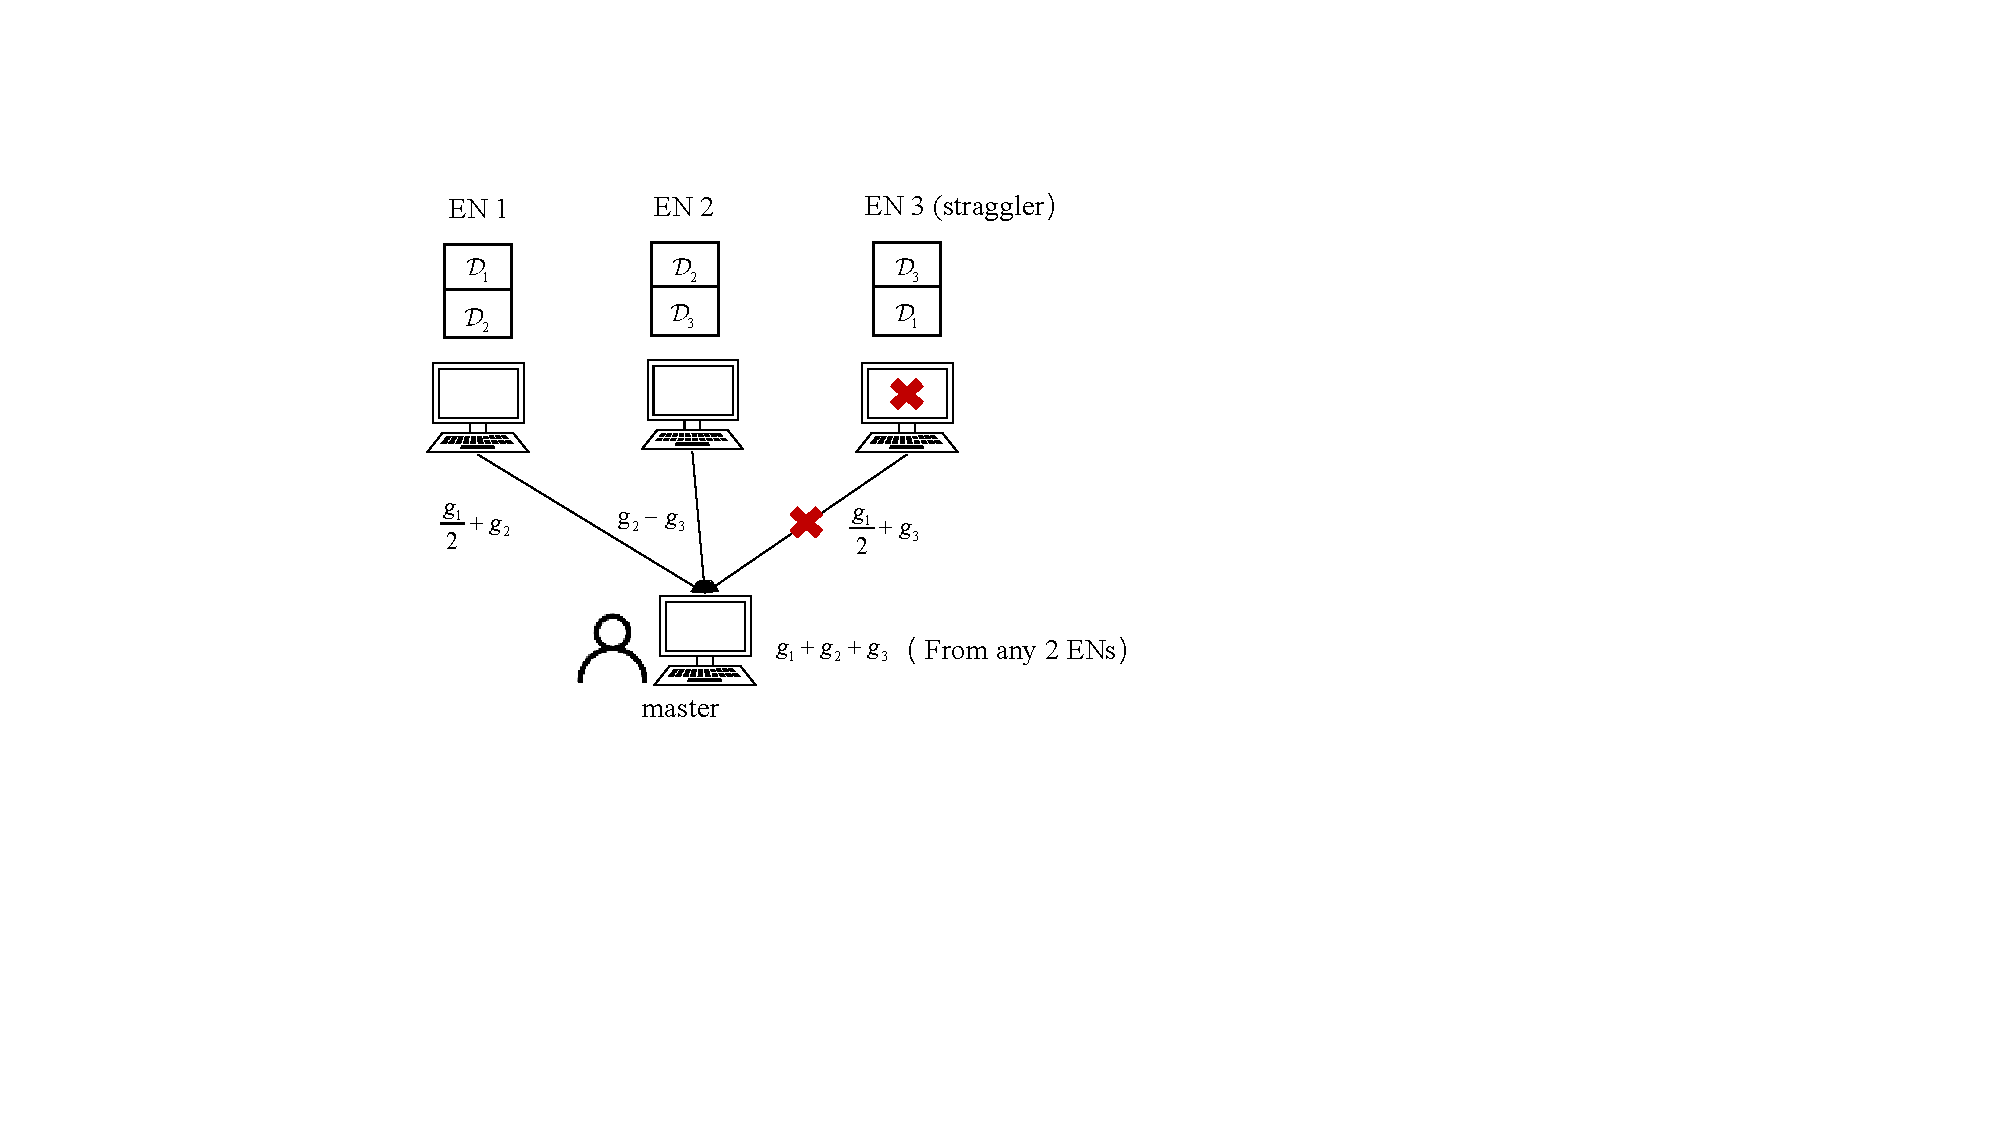
\includegraphics[width=0.5\textwidth]{gradient_coding.pdf}
	\caption{梯度编码计算}
	\label{gradient coding_chapter}
\end{figure}

\subsection{梯度编码计算模型}

%计算完成后，该梯度编码$\tilde{\mathbf{g}}_n^{(t)}$将被回传至移动设备，假设每个元素的梯度结果信息熵为$H(\tilde{g})$。

假设在计算完成时间内，移动设备仅接收到来自非迟滞节点集合$\mathcal{G}\subseteq[N]$的编码梯度$\left\{\tilde{\mathbf{g}}_{k}^{(t)}\right\}_{k\in\mathcal{G}}$。只要完成计算的节点数量满足$|\mathcal{G}|\geq N-S$，梯度编码方案即保证全梯度可恢复。具体来说，移动设备寻找一组解码系数向量$\mathbf{A}_{\mathcal{G}}=\{a_k\}_{k\in \mathcal{G}}$，使得该向量与完成计算的编码矩阵行向量的线性组合等于全$\mathbf{1}$向量，即求解以下线性方程组
\begin{align}
	\sum_{k\in\mathcal{G}}a_k\mathbf{b}_k=\mathbf{1}_{1\times K},
\end{align}
其中$\mathbf{b}_k$是矩阵$\mathbf{B}$的第$k$行，$\mathbf{1}_{1\times K}$是$K$维全1行向量。这确保了对于任意大小为$N-S$的子集，该方程均有解。
求解解码系数$\{\mathbf{a}_n\}_{n\in\mathcal{F}}$后，移动设备通过加权求和接收到的编码梯度来恢复全梯度值
\begin{align}
	\sum_{k\in\mathcal{G}}a_k\tilde{\mathbf{g}}_k^{(t)}=\sum_{k\in\mathcal{G}}a_k\left(\sum_{i=1}^Kb_{k,i}\mathbf{g}_i^{(t)}\right)=\sum_{i=1}^K\left(\sum_{k\in\mathcal{G}}a_kb_{k,i}\right)\mathbf{g}_i^{(t)}=\mathbf{1}\cdot \mathbf{g}_i^{(t)}=\mathbf{g}^{(t)}.
\end{align}
最后，移动设备利用重构的$\mathbf{g}^{(t)}$执行模型参数更新$w^{(t+1)}=w^{(t)}-\lambda \mathbf{g}^{(t)}$，其中$\lambda$表示迭代的步长。

\subsection{下行传输模型}

在计算完成后，从完成计算的节点$\mathcal{G}$中选取信道条件最好的$K$个节点进行传输，记为$\mathcal{K}=\{\pi(1),\cdots,\pi(K)\}$，假设这$K$个节点的信道条件满足$h_{\pi(1)}\geq h_{\pi(2)}\geq \cdots\geq h_{\pi(K)}$。为了提升频谱效率，和上一章节所提传输模型类似，本节也将采用功率域NOMA作为示例，采用其他的多址传输方案例如RSMA也适用。因此，这$K$个节点将被选取参与下行传输，第$k$个边缘节点的下行传输速率$R_k$可以表示为
\begin{equation}
	R_k=B_d\log_2\left(1+\frac{h_kp_k}{B_dn_0+\sum_{j=i+1}^{r}h_jp_j}\right)\label{sic_chapter_4},~\forall k\in\mathcal{K},
\end{equation}
其中$p_k$表示节点$k$的发射功率，$B_d$表示下行传输的带宽，$n_0$表示噪声功率。
类似地，在下行传输前，通常需要将计算结果进行信源编码，$K$个节点的信源编码速率$\tilde{R}_{c,i}$'s和传输速率$R_i$'s 需要满足
\begin{align}
	R_iT_d\geq\tilde{R}_{c,i} s,~\forall i\in\mathcal{K} \label{rt>l}
\end{align}
其中$T_d$表示下行传输延迟，$s$表示每个节点需要传输的梯度计算结果包含的符号数。

本研究旨在提升梯度编码场景中下行传输效率，降低传输时延。传统的传输方案往往会在传输之前对局部梯度值进行信源编码，一些工作采用直接编码方案，即只要信源编码速率满足
\begin{equation}
	\tilde{R}_{c,i}\geq H(\tilde{g}_i),~\forall i\in \mathcal{K}.
\end{equation}
然而，这种直接编码方案将边缘节点下行传输过程视为独立传输过程，并未有效利用节点间计算结果的相关性。由于梯度编码场景中，移动设备需要恢复局部梯度和，如果采用上一章所述的SW定理进行信源编码，本质上仍是恢复局部梯度$\tilde{\mathbf{g}}_k^{(t)}$（$k\in\mathcal{K}$）的值，再利用解码矩阵进行全梯度恢复。如果在信源编码阶段按照线性恢复的方案进行压缩，或许能进一步对局部梯度进行压缩，从而减少冗余信息的传输，提升传输效率。为此，本研究进一步提出了面向线性恢复的DSC辅助编码计算下行传输机制，通过嵌套线性码实现局部梯度值的分布式信源压缩，达到比独立恢复更大的压缩区域，从而提升编码效果。

\subsection{面向线性恢复的 DSC 辅助传输机制}\label{4.3}
本节将详细阐述所提面向线性恢复的DSC辅助编码计算结果下行传输机制，进一步建立下行传输时延优化问题。由于梯度编码场景中，每次迭代$t$移动设备仅需恢复梯度和$\mathbf{g}^{(t)}$。在选取的$K\in \mathcal{K}$个边缘节点传输局部梯度值之前，考虑采用基于嵌套线性码实现的信源编码方案\upcite{lim2019towards}。在无损且无边信息条件下，下面的定理给出了该方案能达到的信源编码速率区域。

\begin{theorem}\label{bcst}
	速率元组$(\tilde{R}_{c,1},\cdots,\tilde{R}_{c,K})$是可达的，只要它包含在以下区域$\mathcal{h}_{lossless}$中
	\begin{equation}
		\mathcal{h}_{lossless}=\bigcup_{\mathbf{E}}\bigcap_{\mathbf{C}}\bigcup_{\mathcal{S}}\bigcap_{\mathcal{T}}\left\{(\tilde{R}_{c,1},\cdots,\tilde{R}_{c,K})\in \mathbb{R}_+^K: \sum_{i\in\mathcal{T}}\tilde{R}_{c,i}>H(\hat{\mathbf{g}}_{\mathbf{E}}|\hat{\mathbf{g}}_{\mathbf{C}\mathbf{E}})\right\},\label{lossless_region}
	\end{equation}
	其中$\hat{\mathbf{g}}_{\mathbf{E}}^{(t)}=\mathbf{E}[\tilde{\mathbf{g}}_1,\cdots,\tilde{\mathbf{g}}_K]^T$，$\hat{\mathbf{Y}}_{\mathbf{C}\mathbf{E}}=\mathbf{C}\mathbf{E}[\tilde{\mathbf{g}}_1,\cdots,\tilde{\mathbf{g}}_K]^T$，集合运算是针对所有满足以下约束的元组（$\mathbf{E},\mathbf{C},\mathcal{S},\mathcal{T}$）进行的
	
	（a）$\mathbf{E}\in \mathbb{F}_q^{L_{\mathbf{E}\times K}}$遍历所有满秩矩阵，使得$1\leq L_{\mathbf{E}}\leq K$且span($\mathbf{E}$)$\supseteq$span($\tilde{\mathbf{F}}$)。
	
	（b）$\mathbf{C}\in \mathbb{F}_q^{L_{\mathbf{C}}\times L_{\mathbf{E}}}$遍历所有满秩矩阵（包括空矩阵），使得$0\leq L_{\mathbf{C}}< L_{\mathbf{E}}$。
	
	（c）$\mathcal{S}\subseteq[1:L_{\mathbf{E}}]$遍历所有大小为$|\mathcal{S}|=L_{\mathbf{E}}-L_{\mathbf{C}}$且满足
	\begin{equation}
		\textrm{rank}\left(\left[\begin{matrix}
			C\\
			\textbf{\textrm{I}}_{L_{\mathbf{E}}}(\mathcal{S})
		\end{matrix}\right]\right)=L_{\mathbf{E}},\label{rankc}
	\end{equation}
	
	（d）$\mathcal{T}\subset[K]$ 遍历所有大小为$|\mathcal{T}|=L_{\mathbf{E}}-L_{\mathbf{C}}$且满足
	\begin{equation}
		\textrm{rank}\left(\left[\begin{matrix}
			\mathbf{E}(\mathcal{S})\\
			\textbf{\textrm{I}}_K([K] \backslash \mathcal{T})
		\end{matrix}\right]\right)=K.\label{ranke}
	\end{equation}
	
\end{theorem}

%考虑文献\cite{lim2019towards}提出的基于代数网络信息论的嵌套信源编码方法，针对梯度编码场景中恢复结果是计算任务的线性组合，无损恢复且无边信息，完全恢复目标函数信源编码方法和经典SW定理不同，嵌套信源编码方法的可达区域为
%\begin{align}
%	\mathcal{h}_{comp}=\bigcup_{\mathbf{E}}\bigcap_{\mathbf{C}}\bigcup_{\mathcal{S}}\bigcap_{\mathcal{T}}\left\{(\eta_{\pi(1)},\cdots,\eta_{\pi(r)})\in \mathbb{R}_+^r: \sum_{i\in\mathcal{T}}\eta_i>H(\hat{\mathbf{Y}}_E|\hat{\mathbf{Y}}_{\mathbf{C}\mathbf{E}})\right\},\label{bcst}
%\end{align}
%其中，$\hat{\mathbf{Y}}_{\mathbf{E}}=\mathbf{E}[\mathbf{g}_{\pi(1)}^{(t)},\cdots,\mathbf{g}_{\pi(r)}^{(t)}]^T, \hat{\mathbf{Y}}_{\mathbf{C}\mathbf{E}}=\mathbf{C}\mathbf{E}[\mathbf{g}_{\pi(1)}^{(t)},\cdots,\mathbf{g}_{\pi(r)}^{(t)}]^T$，且所有元组（$\mathbf{E},\mathbf{C},\mathbf{\mathcal{S}},\mathbf{\mathcal{T}}$）满足定理\ref{<theorem-chapter-4>}中的(b)-(d)以及
%
%（a）$\mathbf{E}\in \mathbb{F}_q^{L_{\mathbf{E}\times r}}$遍历所有满秩矩阵，使得$1\leq L_{\mathbf{E}}\leq r$且span($\mathbf{E}$)$\supseteq$span($\mathbf{F}$)。
%
%因此，在节点完成计算结果后，采用文献\cite{lim2019towards}中的信源编码方案进行信源压缩，可以实现(\ref{bcst})达到的信源压缩区域。

\begin{remark}
定理\ref{bcst}是定理\ref{<theorem-chapter-2>}应用在梯度编码场景中的简化形式，即不考虑边信息且能够无损恢复信源。
\end{remark}

% \subsection{任务总执行时延推导}

\subsection{最小化下行传输时延优化问题}

基于嵌套线性码（具体编码方案详见附录\ref{<nested linear coding>}）构成的信源压缩区域，边缘节点可以根据信道条件调整其压缩率。相应的优化问题可以建模如下
\begin{align}
	\mathcal{P}_{4.1}:& \min_{\mathbf{R},\mathbf{p}, \tilde{\mathbf{R}}_{c},T_d} ~T_{d}\\
	\text{s.t.}~ &(\ref{sic_chapter_4}),(\ref{rt>l}),(\ref{lossless_region}),(\ref{rankc}),(\ref{ranke})\notag,\\
	& 0\leq p_i\leq P_{max}, \label{pmax}~\forall i\in \mathcal{G},
\end{align}
其中 $\mathbf{R} = [R_{\pi(1)}, R_{\pi(2)}, \cdots, R_{\pi(K)}]$, $\mathbf{p} = [p_{\pi(1)}, p_{\pi(2)}, \cdots, p_{\pi(K)}]$, 以及 $\tilde{\mathbf{R}}_{c}=[\tilde{R}_{c,1},\cdots,\tilde{R}_{c,K}]$ 是相应变量的紧凑表示；$P_{max}$ 是每个 节点的最大发射功率；

\begin{remark}
	相比于经典Slepian-Wolf定理的信源可达区域，在梯度编码场景中，移动设备不用恢复完整子任务的计算结果，再将计算结果进行求和，而只需要恢复线性组合。利用嵌套线性码可以达到各节点信源压缩时按照线性特定关系进行编码压缩，从而达到比恢复各节点计算结果更大的压缩区域，因此扩大了优化区域。
\end{remark}

\section{面向线性恢复的DSC辅助编码计算结果传输算法}\label{4.4}
由于问题$P_{4.1}$直接利用区域$\mathcal{h}_{lossless}$进行优化，需要遍历满足（a）-（d）所有的情况，增加优化问题的复杂度，为了保证优化的区域以及优化问题求解的复杂度不会过高，可以利用边界条件进行简化。
\begin{theorem}\label{<linear>}
	针对面向线性恢复的计算结果下行传输场景，基于嵌套线性码的低复杂度可达速率区域$\mathcal
	h_{sub}$定义为独立数据恢复边界$\mathcal{h}_{sw}$与线性直接恢复边界$\mathcal{h}_{linear}$的并集
	\begin{equation}
		\mathcal{h}_{sub} \triangleq \mathcal{h}_{sw} \cup \mathcal{h}_{linear},
	\end{equation}
	其中，
	\begin{align}
		&\mathcal{h}_{sw}=\left\{(\tilde{R}_{c,k}):\sum_{k\in\mathcal{L}}\tilde{R}_{c,k}>H\left(\{\mathbf{\tilde{g}}_k\}_{k\in\mathcal{L}}|\{\mathbf{\tilde{g}}_n\}_{n \notin\mathcal{L}}\right), \forall \mathcal{L}\subseteq \mathcal{K}\right\},\label{hsw}\\
		&\mathcal{h}_{linear}=\left\{(\tilde{R}_{c,k}): \tilde{R}_{c,k}>H\left(\mathbf{g}^{(t)}\right),\forall k\in \mathcal{K}\right\}.\label{hlinear}
	\end{align}
	任何落在该并集区域内的速率元组均可实现全梯度$\mathbf{g}^{(t)}$的无损重构。
\end{theorem}
\begin{proof}
	推导见附录\ref{<linear-proof>}。
\end{proof}

因此，问题$P_{4.1}$可以近似简化为
\begin{align}
		\mathcal{P}_{4.2}:& \min_{\mathbf{R},\mathbf{p}, \tilde{\mathbf{R}}_{c},T_d} ~T_{d}\\
	\text{s.t}.~ &(\ref{sic_chapter_4}),(\ref{rt>l}),(\ref{pmax}),(\ref{hsw}), (\ref{hlinear})\notag.
\end{align}
更进一步，可以将信源压缩区域拆分成两个子区域分别进行优化，即问题$P_{4.2}$可以等价的分为$P_{4.3}$和$P_{4.4}$的最小值，即$P_{4.2}=\min \left\{P_{4.3},P_{4.4}\right\}$，其中$P_{4.3}$和$P_{4.4}$可以分别表示为
\begin{align}
	\mathcal{P}_{4.3}:& \min_{\mathbf{R},\mathbf{p}, \tilde{\mathbf{R}}_{c},T_d} ~T_{d}\\
	\text{s.t}.~ &(\ref{sic_chapter_4}),(\ref{rt>l}),(\ref{pmax}),(\ref{hsw})\notag.
\end{align}
以及
\begin{align}
	\mathcal{P}_{4.4}:& \min_{\mathbf{R},\mathbf{p}, \tilde{\mathbf{R}}_{c},T_d} ~T_{d}\\
	\text{s.t}.~ &(\ref{sic_chapter_4}),(\ref{rt>l}),(\ref{pmax}), (\ref{hlinear})\notag.
\end{align}

类似地，由于子问题$P_{4.3}$和子问题$P_{4.4}$都是非凸问题，与第三章算法类似，可以通过转换为凸差问题，使用CCCP技术求解。具体来说，公式（\ref{sic_chapter_4}）以及公式（\ref{rt>l}）同样可以通过引入辅助变量$\{\mu_i\}_{i=1}^K$以及$\{\nu_i\}_{i=1}^K$，等价转为DC形式
\begin{subnumcases}
	{}\nu_i=\frac{1}{2}\left(R_i+T_d\right),~\forall i\in\mathcal{K},\label{zc}\\
	\mu_i=\frac{1}{2}(R_i-T_d),~\forall i\in\mathcal{K},\label{xc}\\
	\nu_i^2-\mu_i^2- \tilde{R}_{c,i}s\geq 0,~\forall i\in\mathcal{K}.\label{zxc}
\end{subnumcases}
公式(\ref{sic_chapter_4})已经是一个DC形式的约束，因此问题$\mathcal{P}_{4.3}$和$\mathcal{P}_{4.4}$可以等价转化为
\begin{align}
	\mathcal{P}_{4.5}:& \min_{\mathbf{R},\mathbf{p}, \tilde{\mathbf{R}}_{c},T_d} ~T_{d}\\
	\text{s.t}.~ &(\ref{sic_chapter_4}),(\ref{pmax}),(\ref{hsw}),(\ref{zc}),(\ref{xc}),(\ref{zxc})\notag.
\end{align}
以及
\begin{align}
	\mathcal{P}_{4.6}:& \min_{\mathbf{R},\mathbf{p}, \tilde{\mathbf{R}}_{c},T_d} ~T_{d}\\
	\text{s.t}.~ &(\ref{sic_chapter_4}),(\ref{pmax}), (\ref{hlinear}),(\ref{zc}),(\ref{xc}),(\ref{zxc})\notag.
\end{align}
求解$\mathcal{P}_{4.5}$和$\mathcal{P}_{4.6}$可以利用CCCP算法。在第$(\tau+1)$次迭代中，利用第$\tau$次迭代得到的最优解（$\mathbf{R}^{(\tau)},\mathbf{p}^{(\tau)},\symbfit{\nu}^{(\tau)},\symbfit{\mu}^{(\tau)},\tilde{\mathbf{R}}_{c}^{(\tau)}$），对约束中的凹部分进行线性化近似求解，其中$\mathbf{R}^{(\tau)}=[R_1^{(\tau)},\cdots,R_{K}^{(\tau)}],\mathbf{p}^{(\tau)}=[p_1^{(\tau)},\cdots,p_{K}^{(\tau)}],\symbfit{\mu}^{(\tau)}=[\mu_1^{(\tau)},\cdots,\mu_{K}^{(\tau)}],\symbfit{\nu}^{(\tau)}=[\nu_1^{(\tau)},\cdots,\nu_{K}^{(\tau)}],$$\mathbf{R}_{c}^{(\tau)}=[R_{c,1}^{(\tau)},\cdots,R_{c,K}^{(\tau)}]$为优化变量的向量形式。具体而言，第（$\tau$+1）次迭代中（\ref{zxc}）可以近似为
\begin{equation}
		\mu_i^2-\left(\left({\nu_i}^{(\tau)}\right)^2+2\nu_i^{(\tau)}\left(\nu_i-\nu_i^{(\tau)}\right)\right)
	+ \tilde{R}_{c,i}s\leq 0,~ \forall i\in\mathcal{K}.\label{cccp3}
\end{equation}
类似的，（\ref{sic_chapter_4}）的凹部分可以参考第三章（\ref{cccp2}）进行线性化
	\begin{align}
	R_i\geq &
	B_d\log_2\left({B_dn_0+\sum\nolimits_{j={i}}^{K}h_jp_j}\right)
	-B_d\log_2\left({B_dn_0+\sum\nolimits_{j={i+1}}^{K}h_jp_j^{(\tau)}}\right)\notag\\&-
	B_d\left(\frac{\sum_{j={i+1}}^{K}h_j\left(p_{j}-p_{j}^{(\tau)}\right)}{(\ln2)\left(\sum_{j={i+1}}^{K}h_jp_{j}^{(\tau)}+Bn_0\right)}\right),~\forall i\in\mathcal{K}\label{cccp4}.
\end{align}
因此，在第$(\tau+1)$次迭代中，$\mathcal{P}_{4.5}$和$\mathcal{P}_{4.6}$可以近似转化为如下凸问题
\begin{align}
	\mathcal{P}_{4.7}:& \min_{\mathbf{R},\mathbf{p}, \tilde{\mathbf{R}}_{c},T_d} ~T_{d}\\
	\text{s.t}.~ &(\ref{pmax}),(\ref{hsw}),(\ref{zc}),(\ref{xc}),(\ref{cccp3}),(\ref{cccp4})\notag.
\end{align}
以及
\begin{align}
	\mathcal{P}_{4.8}:& \min_{\mathbf{R},\mathbf{p}, \tilde{\mathbf{R}}_{c},T_d} ~T_{d}\\
	\text{s.t}.~ &(\ref{pmax}), (\ref{hlinear}),(\ref{zc}),(\ref{xc}),(\ref{cccp3}),(\ref{cccp4})\notag.
\end{align}
$\mathcal{P}_{4.7}$和$\mathcal{P}_{4.8}$可以通过标准方法求解，具体过程见算法1。

\begin{algorithm}[h]
	%				\footnotesize
	\caption{面向线性恢复的DSC辅助编码计算结果下行传输算法}
	%			\begin{algorithmic}[1]
%		\SetKwInOut{Input}{输入}\SetKwInOut{Output}{输出}
		\SetKwRepeat{Repeat}{repeat}{until}%
		\LinesNumbered
%		\Input{容差 $\epsilon$, 功率约束 $P_{max}$,任务包大小 $l$;}
%		\Output{传输速率 $\mathbf{R}^*$, 发射功率 $\mathbf{p}^*$, 信源压缩率 $\symbfit{\eta}^*$, 下行传输延迟 $T_d^*$;}
		初始化：算法收敛精准度$\epsilon$，发射功率约束$P_{max}$，传输包符号数$s$;\\
		选择一个初始可行点 ($\mathbf{p}_{sw}^{(0)}$, $\symbfit{\nu}_{sw}^{(0)}$) ，并设置迭代次数 $\tau=1$;\\
		\Repeat{$|T_{d_{sw}}^{(\tau)}-T_{d_{sw}}^{(\tau-1)}|\leq \epsilon$}{
			基于 $\left\{\left(\mathbf{R}_{sw}^{(\tau)},\mathbf{p}_{sw}^{(\tau)},\symbfit{\nu}_{sw}^{(\tau)},\symbfit{\mu}_{sw}^{(\tau)},\symbfit{\bar{\eta}}_{sw}^{(\tau)}\right)\right\}$求解 $\mathcal{P}_{4.7}$ ;\\
			计算 $T_{d_{sw}}^{(\tau+1)}$;\\
			令 $\tau=\tau+1$;}
		\Repeat{$|T_{d_{linear}}^{(\tau)}-T_{d_{linear}}^{(\tau-1)}|\leq \epsilon$}{
			 基于 $\left\{\left(\mathbf{R}_{linear}^{(\tau)},\mathbf{p}_{linear}^{(\tau)},\symbfit{\nu}_{linear}^{(\tau)},\symbfit{\mu}_{linear}^{(\tau)},\symbfit{\bar{\eta}}_{linear}^{(\tau)}\right)\right\}$求解 $\mathcal{P}_{4.8}$;\\
			计算 $T_{d_{linear}}^{(\tau+1)}$;\\
			令 $\tau=\tau+1$;}
			\If{$T_{d_{linear}}<T_{d_{sw}}$}
			{\text{返回}\quad$\mathbf{R}^*=\mathbf{R}_{linear}^{(\tau)}$, $\mathbf{p}^*=\mathbf{p}_{linear}^{(\tau)}$, $\symbfit{\eta}^*=\symbfit{\eta}_{linear}^{(\tau)}$, $T_d^*=T_{d_{linear}}^{(\tau)}$.}
		\Else
		{\text{返回}\quad$\mathbf{R}^*=\mathbf{R}_{sw}^{(\tau)}$, $\mathbf{p}^*=\mathbf{p}_{sw}^{(\tau)}$, $\symbfit{\eta}^*=\symbfit{\eta}_{sw}^{(\tau)}$, $T_d^*=T_{d_{sw}}^{(\tau)}$.}
		
		%			\end{algorithmic}	
\end{algorithm}

\begin{corollary}\label{condition}
	考虑特殊情况，即所有完成计算节点的下行传输信道条件相同时，当且仅当全梯度的熵$H(\mathbf{g}^{(t)})$与局部编码梯度的联合熵$H(\left\{\tilde{\mathbf
	{g}}_k\right\}_{k\in\mathcal{K}})$满足以下条件时，采用线性直接恢复压缩策略$\mathcal{h}_{linear}$比经典Slepian-Wolf策略$\mathcal{h}_{sw}$具有更低的传输延迟
	\begin{align}
		H(\left\{\tilde{\mathbf{g}}_k\right\}_{k\in\mathcal{G}})>r \cdot H(\mathbf{g}^{(t)}).
	\end{align}
	直观理解，该条件意味着梯度编码引入的数据冗余度与局部噪声之比超过了完成计算节点的数量。
\end{corollary}
\begin{proof}
	证明详见证明\ref{<condition>}。
\end{proof}


\section{仿真性能与分析}\label{4.5}
本节将通过数值仿真验证所提机制的有效性。
在仿真中，对于下行传输，采用瑞利衰落信道模型 $h_i = |\mathbf{h}_i|^2 \rho$ \cite{goldsmith2005wireless}，其中 $\rho$ 为平均增益，小尺度衰落系数 $\mathbf{h}_i$ 服从复高斯分布 $\mathcal{CN}(0, 1)$。
噪声功率谱密度 $n_0$ 设定为 $1 \times 10^{-17}$ (W/Hz)，下行信道带宽 $B$ 设定为 20 (MHz)。
此外，由于嵌套线性码的性能与我们的工作是正交的，假设采用理想的嵌套线性码实现无损恢复。完成计算并参与下行传输的 $K$ 个 边缘节点是随机选择的，并基于这些选择的 节点执行 $1 \times 10^4$ 次蒙特卡洛运行以获得平均性能。梯度编码中，考虑采用循环重复编码方案，分别考虑两种场景：一是边缘节点数目与子任务划分数目相等，均为$N=5$，恢复阈值为$K=3$，二是边缘节点数目与子任务划分数目相等，均为$N=7$，恢复阈值为$K=4$。
为了验证所提机制的有效性，本节通过仿真实验对比了以下两种基线方案的性能：
 基线方案一考虑传统信源独立编码方式，即各边缘节点独立传输计算结果，不进行分布式信源编码压缩。基线方案二考虑采用理论 SW编码对各边缘节点进行分布式信源压缩，利用 SW 理论区域进行完整数据恢复的压缩传输方案。



\begin{figure}[htbp]
    \centering
    \includegraphics[width = 0.75 \textwidth]{figs/real_channel_gain_Chinese.eps}
    \caption{不同平均信道增益$\rho$下的下行传输时延$T_d$比较（最大发射功率约束$P_{max}=0.2$（W））。}
    \label{fig:4.2}
\end{figure}

图~\ref{fig:4.2}展示了在不同平均信道功率增益$\rho$下，分别对参数$N=5$和$K=3$以及$N=7$和$K=4$对平均下行传输时延$T_d$的性能比较。可以观察到，利用理论SW编码方案和所提基于线性码的线性恢复编码方案相比于基线方案一都有明显的性能提升。例如，当平均信道增益为$\rho=-115$（dB）且参数$N=5,K=3$的场景下，所提面向线性恢复传输方案的下行平均传输延迟为$0.078$（ms），基线方案二面向独立恢复传输方案的下行平均传输延迟为$0.084$（ms），都比基线方案一独立传输方案的下行平均延迟$0.097$（ms）低，且所提方案相比于基线方案二也降低了传输延迟，这是由于所提方案在面向计算结果线性恢复的场景中，利用嵌套线性码能够达到更大的信源编码区域，从而达到更好的负载重分配的效果。当平均信道增益为$\rho=-115$（dB）且参数$N=7,K=4$的场景下，所提面向线性恢复传输方案相比于基线方案一的性能增益为$49\%$，相比于基线方案二的性能增益为$6\%$。可以看出，当节点数增加后，相比于基线方案一，所提方案有了更明显的性能提升。这是因为，当节点数增加后，信道条件差的节点出现的概率增大。基线方案一中每个节点独立传输，如果其中一个节点的信道条件较差，会影响整体的传输延迟。而所提方案采用了面向线性恢复的DSC方案，可以实现节点间传输负载的重分配效果，使得信道条件差的节点少传一部分信息，信道条件好的节点多传一部分信息，从而避免了单个节点影响整体传输性能。


\begin{figure}[htbp]
	\centering
	\includegraphics[width = 0.75 \textwidth]{figs/real_transmit_power_Chinese.eps}
	\caption{不同最大发射功率$P_{max}$下的下行传输时延$T_d$比较（平均信道增益为$\rho=-110$（dB）。}
	\label{fig:4.3}
\end{figure}
图~\ref{fig:4.3}展示了在不同最大发射功率$P_{max}$下，分别对参数$N=5$和$K=3$以及$N=7$和$K=4$对平均下行传输时延$T_d$的性能比较。可以观察到，所提方案相比于基线方案仍然有显著的性能增益。例如，当$P_{max}=0.05$（W）且参数$N=5,K=3$的场景下，所提方案相比于基线方案一的性能增益为$50\%$，相比于基线方案二的性能增益为$8\%$。当$P_{max}=0.05$（W）且参数$N=7,K=4$的场景下，所提方案相比于基线方案一的性能增益为$58\%$，相比于基线方案二的性能增益为$14\%$。此外，当最大发射功率越小时，性能增益越明显。例如，当$P_{max}=0.45$（W）且参数$N=5,K=3$的场景下，所提方案相比于基线方案一的性能增益为$42\%$，当参数$N=7,K=4$的场景下，所提方案相比于基线方案一的性能增益为$37\%$。进一步验证了，当信道条件差的情况下，所提方案能够提供更灵活的信源编码区域，达到负载重分配的效果。


%图~\ref{fig:4.2} 和图~\ref{fig:4.4} 展示了在不同平均信道功率增益 $\rho$ 下，平均任务执行时延 $T_d$ 的性能比较。其中图例分别展示了两种不同的系统配置：配置一为 $r=3, k=5$（实心点曲线），配置二为 $r=4, k=7$（空心点曲线）。可以观察到，随着信道条件 $\rho$ 的改善（从 $-115\text{ dB}$ 增加到 $-105\text{ dB}$），所有方案的时延均显著降低。然而，在相同的信道条件下，本文提出的基于代数嵌套线性码的方案始终优于基准方案和基于理想 SW 码的方案。例如，在 $\rho = -115\text{ dB}$ 且 $r=3, k=5$ 的情况下，基准方案的时延约为 $160\text{ ms}$，理想 SW 方案的时延约为 $125\text{ ms}$，而采用代数嵌套线性码的方案时延仅为 $105\text{ ms}$ 左右。这证实了定理 4.3 的结论，即针对梯度聚合等线性计算任务，直接恢复函数值的压缩效率要高于恢复完整原始数据，从而能获得更大的可达速率区域和更低的传输时延。此外，相比于独立传输的基准方案，所提方案利用了重复计算引入的冗余信息进行协作传输，有效缓解了深衰落节点对系统性能的限制。
\begin{figure}[htbp]
	\centering
	\includegraphics[width = 0.75 \textwidth]{figs/equal_channel_gain_Chinese.eps}
	\caption{边缘节点信道条件相同，不同平均信道增益$\rho$下的下行传输时延$T_d$比较（最大发射功率约束$P_{max}=0.2$（W））。}
	\label{fig:4.4}
\end{figure}
图~\ref{fig:4.4}展示了边缘节点平均信道功率增益相同的情况下，平均下行传输时延$T_d$的性能比较。类似地可以观察到，当信道条件越差时，所提方案相较于基线方案一的性能增益越明显。例如，当参数$N=5,K=3$的场景下，$\rho=-105$（dB）时，所提方案对比基线方案一的性能增益为$29\%$，当$\rho=-115$（dB）时，所提方案对比基线方案的性能增益为$30\%$。当参数$N=7,K=4$的场景下，$\rho=-105$（dB）时，所提方案对比基线方案一的性能增益为$37\%$，当$\rho=-115$（dB）时，所提方案对比基线方案的性能增益为$38\%$。
在信道条件相同的情况下，随着信道条件越差 所提方案相比于基线方案二的性能增益也有所提升。例如，当参数$N=5,K=3$的场景下，$\rho=-105$（dB）时，所提方案相比于基线方案二的性能增益为$8\%$，当$\rho=-115$（dB）时，所提方案相比于基线方案二的性能增益为$11\%$。这是由于所提方案的DSC可行域比基线方案二的DSC区域多出来一个拐点，即与推论\ref{condition}所给出的内容一致，验证了所提方案相比基线方案二的性能优势。

图~\ref{fig:4.5}展示了边缘节点平均信道功率相同的情况下（$\rho=-110$（dB）），比较不同最大发射功率$P_{max}$条件下的下行传输时延$T_d$。类似地可以观察到当$P_{max}=0.05$（W）时，所提方案相比于基线方案一的性能增益在$N=5,K=3$和$N=7,K=4$场景下分别为$26\%$和$24\%$。所提方案相比于基线方案二的性能增益在$N=5,K=3$和$N=7,K=4$场景下分别为$7\%$和$8\%$。
\begin{figure}[htbp]
	\centering
	\includegraphics[width = 0.65 \textwidth]{figs/equal_transmit_power_Chinese.eps}
	\caption{边缘节点信道条件相同，不同最大发射功率$P_{max}$下的下行传输时延$T_d$比较（平均信道增益为$\rho=-110$（dB）。}
	\label{fig:4.5}
\end{figure}



%图~\ref{fig:4.3} 和图~\ref{fig:4.5} 展示了边缘节点最大传输功率 $P_{\max}$ 对平均任务执行时延的影响。从图中可以看出，随着发射功率预算的增加，下行传输速率提升，从而降低了总时延。在低功率区域（如 $P_{\max}=0.05\text{ W}$），所提方案的优势尤为明显。对比图中 $r=3, k=5$ 的情况，当 $P_{\max}=0.05\text{ W}$ 时，基于代数嵌套线性码的方案相较于基准方案降低了约 50\% 以上的时延。这是因为在功率受限的情况下，通信资源更为稀缺，本文提出的方案通过更高效的信源压缩（嵌套线性码）和功率分配优化，能够在有限的功率预算下实现更快速的结果汇聚。同时，图中的放大子图进一步清晰地展示了在高功率区域，虽然各方案间差距缩小，但所提方案依然保持了最低的时延性能，证明了其在不同信噪比环境下的鲁棒性。
%
%
%
%综合图~\ref{fig:4.2} 至图~\ref{fig:4.5} 的结果，可以得出结论：在分布式边缘计算的梯度聚合场景中，利用计算结果间的代数结构相关性，采用面向线性恢复的分布式信源编码策略，能够突破传统 Slepian-Wolf 编码的性能瓶颈，显著降低下行协作传输的时延。


\section{本章小结}\label{chapter-sum}
本章针对编码计算中计算结果下行传输过程由于可能存在信道深衰落造成的通信瓶颈问题，提出了一种面向线性恢复的DSC辅助下行传输机制。与现有将下行传输视为独立多用户通信的研究不同，本研究综合考虑了任务编码引入的计算冗余与通信阶段的协作传输增益之间的权衡。
针对梯度下降等线性聚合类任务，不再局限于恢复单个子任务的计算结果，而是利用嵌套线性码，构建了面向线性函数恢复的传输模型。理论分析表明，相比于经典的 SW定理完整重构信源，面向线性恢复的编码策略拥有更大的可达压缩区域。在此基础上，建立了以最小化任务总执行时延为目标的优化问题，并利用交替优化和差分凸规划算法联合优化了任务划分与下行传输功率分配。
仿真结果表明，所提出的基于代数嵌套线性码的DSC辅助下行传输方案在时延性能上显著优于传统的独立传输方案以及基于 SW定理 的完整恢复方案，特别是在信道条件较差或功率受限的场景下，能够有效降低系统的下行传输时延，提升编码计算整体处理任务的效率。